\section{Verwaltung von Testdaten und -systemen}\label{chap:testdataadministration}

%%%%%%%%%%%%%%%%
%
%    Verwaltung von Test-Daten und Test-Systemen
%
%%%%%%%%%%%%%%%%

An das Backend der Web-IDE ist eine eigene SAP HANA-Instanz angebunden.
Darin werden die Testdatensets und Zugangsdaten für Testsysteme hinterlegt.
Im Folgenden geht es um das zugrundeliegende Schema, die Integration verschiedener Testsysteme und das Pflegen der Testdaten, insbesondere in Hinblick auf deren Gültigkeit.

\subsection{Datenschema für Testdatensets}
Die größte Herausforderung beim Speichern der Testdatensets liegt in der Wiederzuordnung zu den Variablen in der vom Entwickler geöffneten Quellcodedatei.
Der in der Web-IDE genutzte Quellcode-Parser \cite{Horschig2014} nutzt symbolische Ausführung \cite{DBLP:journals/cacm/King76} zur Bestimmung von Variablen und deren eventuell bereits festgelegten Werten.
Die auf diesem Wege gefundenen Variablen bekommen eine eindeutige Kennzeichnung, die zum Identifizieren genutzt werden kann.
Sollten die Variablen im Laufe des Programmflusses in mindestens ein SQL-Statement einfließen, werden sie als sog. Testvariablen betrachtet.
Eine Menge von Testvariablen bildet zusammen mit dem Pfad der geöffnet Quellcodedatei auf dem Server und einem vom Entwickler angegebenen Namen ein Testdatenset.
Diese Sets können wiederum in Beziehung mit dem Testsystem gebracht werden, auf dem die Performance-Analysen erfolgten, um die Abhängigkeit der Systemauswahl auf die Laufzeiten der Testdatensets zu berücksichtigen.
In Abbildung \ref{fig:erm} ist das dazugehörige Datenschema dargestellt.

\newcommand {\key}[1]{\underline{#1}}

\begin{figure}[ht]
	\centering
	\begin{tikzpicture}[node distance = 7em]
		\node [entity] (testset) {Test Set};
		\node [attribute] (tsid) [left of=testset] {\key{ID}} edge (testset);
		\node [attribute] (tsname) [above right of=testset] {Name} edge (testset);
		\node [attribute] (tsfilepath) [above left of=testset] {File Path} edge (testset);
		\node [relationship] (tshastv) [right of=testset] {has} edge (testset);
		\node [entity] (testvalue) [right of=tshastv] {Test Variable} edge [total] (tshastv);
		\node [attribute] (tvid) [above left of=testvalue] {\key{ID}} edge (testvalue);
		\node [attribute] (tvvariable) [above right of=testvalue] {Variable} edge (testvalue);
		\node [attribute] (tvvalue) [right of=testvalue] {Value} edge (testvalue);
		\node [relationship] (tshastsys) [below = 0.5cm of testset] {has} edge (testset);
		\node [entity] (testsystem) [below = 0.5cm of tshastsys] {Test System} edge [total] (tshastsys);
		\node [attribute] (tsysname) [left of=testsystem] {\key{Name}} edge (testsystem);
		\node [attribute] (tsyshost) [below right of=testsystem] {Host} edge (testsystem);
		\node [attribute] (tsysport) [below of=testsystem] {Port} edge (testsystem);
		\node [attribute] (tsysuser) [below left of=testsystem] {User} edge (testsystem);
		\node [attribute] (tsyspassword) [right = 0.5cm of testsystem] {Password} edge (testsystem);
	\end{tikzpicture}
	\caption{ER-Diagramm für die Administration von Testdatensets und -systemen}
	\label{fig:erm}
\end{figure}

\subsection{Caching und Gültigkeit von Testdaten}
Um nicht für jede Vorschlagsanfrage einen Datenbankzugriff durchzuführen, werden die Testdaten und Testdatensets sowohl im Frontend als auch im Backend gecached.
Die Caches unterscheiden sich in der Hinsicht, dass es einen Frontendcache für jede Sitzung eines Entwicklers gibt, wohingegen der Backendcache global agiert.
Eine Anfrage für Testdatenvorschläge zu einer Spalte einer Relation wird dabei erst versucht durch den Frontendcache zu beantworten.
Sollten dort keine passenden Daten vorliegen, wird eine Anfrage an das Backend ausgelöst.
Dort versucht der Backendcache als erste Instanz diese Anfrage zu beantworten.
Sollten auch dort keine Daten vorliegen, werden die Vorschläge mithilfe der in Kapitel \ref{chap:testdatasuggestions} vorgestellten Algorithmen bestimmt und in den Caches hinterlegt.

Eine Herausforderung stellt das Überprüfen der Gültigkeit der Vorschläge und Testdatensets dar.
Diese kann durch zwei Fälle beeinflusst werden: die Daten in der genutzten Datenbank werden verändert (erweitert, aktualisiert oder gelöscht) oder der Quellcode der Anwendung wird in einer Weise abgeändert, die die Variablen aus den SQL-Statements beeinflusst.

Für Ersteres gibt es Ansätze \cite{DBLP:conf/dasfaa/HarangsriSN97}, die kontinuierlich verändernde SQL-Statements nachverfolgen und dementsprechend ihren Algorithmus durch manuelles Mitzählen der Anzahl von Einträgen in der betrachteten Relation anpassen.
Dieser Ansatz ist für die in Kapitel \ref{chap:testdatasuggestions} beschrieben Algorithmen nicht anwendbar, da sie nicht nur die Anzahl der Vorkommen innerhalb einer Relation betrachten, sondern darüber hinaus auch die Werteausprägungen und Analyseergebnisse für die Vorschlagsgenerierung berücksichtigen.
Nichtsdestotrotz floss die Idee der Betrachtung von manipulierenden SQL-Statements mit in die Implementierung ein, indem ein Schwellwert für Datenveränderungen festgelegt wird (derzeit 10), ab dem eine Neubestimmung der Vorschläge und der initial berechneten Testdatensets erfolgt.

Die Invalidierung der Daten durch Veränderung des dazugehörigen Quellcodes wurde im Zuge dieser Arbeit nicht betrachtet, ist aber als Weiterentwicklung geplant.
Die Herausforderung liegt in der Findung einer Granularität, auf der Änderungen zur Invalidierung führen, und gegebenenfalls diese Veränderung nachzuvollziehen.
Legt man die Granularitätsstufe auf das gesamte Dokument fest, würde dies dazu führen, dass die Testdaten zu häufig als ungültig gekennzeichnet werden, obwohl das nicht zwangsläufig zutreffen muss.
Wählt man eine feine Granularitätsstufe (zum Beispiel alle Änderungen, die nur Variablen betreffen, die in SQL-Statements einfließen), so ist eine komplexe Nachverfolgung der Änderungen am Dokument über dessen verschiedene Revisionen notwendig.
Sollte ein Versionsverwaltungssystem für die Quellcodedateien genutzt werden, könnten dessen Informationen in der Nachverfolgung berücksichtigt werden.

\subsection{Integration mehrerer Testsysteme}
Typischerweise dient nicht nur ein System als Grundlage für Performance-Analysen einer Geschäftsanwendung, sondern ein Auswahl an Systemen mit unterschiedlichen Ausstattungsmerkmalen.
Dies kann mehrere Gründe haben.
In Hinblick auf die Daten können so Datenschutzbestimmungen eingehalten oder auch Datensätze mit verschiedene Charakteristiken getestet werden.
Zum anderen kann so auch die Auswirkung verschiedener Systemkonfigurationen auf die Performance der Anwendung geprüft werden, wodurch Kosten gespart werden können, indem man eine passendes System für den Produktiveinsatz auswählt.
Realisiert wird dies durch ein Menü in der Web-IDE (vgl. Abbildung \ref{fig:hanainstances}) bei dem das gewünschte Testsystem ausgewählt oder aber auch neue hinzufügt oder existierende entfernt werden können.
Die Zugangsdaten für die Systeme werden in der Datenbank der Web-IDE hinterlegt (vgl. Abbildung \ref{fig:erm}) und das derzeit vom Entwickler ausgewählte System in seinen Sitzungsdaten gespeichert.
\begin{figure}[ht]
	\centering
  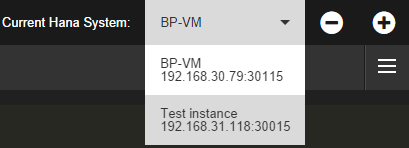
\includegraphics[width=0.6\textwidth]{figures/hana-instances.png}
	\caption{Auswahlmenü für verschiedene Datenbankserver}
	\label{fig:hanainstances}
\end{figure}

